\documentclass[10pt,a4paper]{article}
\usepackage[utf8]{inputenc}
\usepackage[portuges]{babel}
\usepackage{a4wide}
\usepackage{indentfirst}
\usepackage{graphicx}
\usepackage{color}
\usepackage[dvipsnames]{xcolor}

\begin{document}
\title{\bf{\textcolor{Mahogany}{Projeto de Programação Orientada a Objetos}\\ \huge Grupo 30}}

\graphicspath{ {/home/jessica/Desktop/} }
\begin{figure}[t]
    \centering
	\center
\includegraphics[width=4cm]{UM}\\
\end{figure}
\date{maio 2018}
\maketitle
\begin{center}
{\bf{\Huge{JavaFatura}}}

\graphicspath{ {/home/jessica/Desktop/} }
\vspace{6cm}

	\includegraphics[height=3cm]{Marta}  \qquad \qquad \quad
	\includegraphics[height=3cm]{Jessica} \qquad \qquad \quad
	\includegraphics[height=3cm]{Pedro} \qquad 
\end{center}
\begin{center}
\author{ Ana Ribeiro (A82474) \and \qquad Jéssica Lemos (A82061) \and \qquad Pedro Pinto (A82535)}
\end{center}

\thispagestyle{empty}
\cleardoublepage

\thispagestyle{empty}
\tableofcontents
\cleardoublepage
\pagenumbering{arabic}
\setcounter {page}{1}

\section{Introdução}

Este relatório aborda a implementação de uma aplicação capaz de gerir as faturas de um contribuinte. Esta admite dois tipos de entidades: Contribuintes Coletivos e Contribuintes Individuais. Sendo que os primeiros têm a possibilidade de: 

\begin{itemize}
 \item Registar faturas
 \item Aceder às faturas emitidas e às quais emitiu
 \item Associar e alterar a atividade económica às faturas emitidas em seu nome
 \item Obter o montante de dedução fiscal
 \item Obter as faturas emitidas para uma dado contribuinte
 \item Total faturado
\end{itemize}

 \noindent Os Contribuintes Individuais podem:
\begin{itemize}
 \item Aceder às faturas emitidas
 \item Associar e alterar a atividade económica às faturas emitidas em seu nome
 \item Obter o montante de dedução fiscal do próprio e do agregado familiar
\end{itemize}

 \noindent Além destes dois atores existe ainda o Administrador da aplicação que tem acesso a:
\begin{itemize}
 \item 10 contribuintes que mais gastam em todo o sistema
 \item X empresas que mais facturam em todo o sistema
 \item Montante de deduções fiscais que as despesas registadas representam
 \item Número de contribuintes na aplicação
 \item Faturas alteradas pelos contribuintes
\end{itemize}

 \noindent Assim iremos apresentar as classes elaboradas e as relações estabelecidas, bem como o modo de estruturação dos dados. Para tal aplicamos a matéria lecionada até ao momento na respetiva unidade curricular.

\cleardoublepage

\section{Arquitetura de classes}
\label{sec:solucao}


\begin{center}
\graphicspath{ {/home/jessica/Desktop/} }
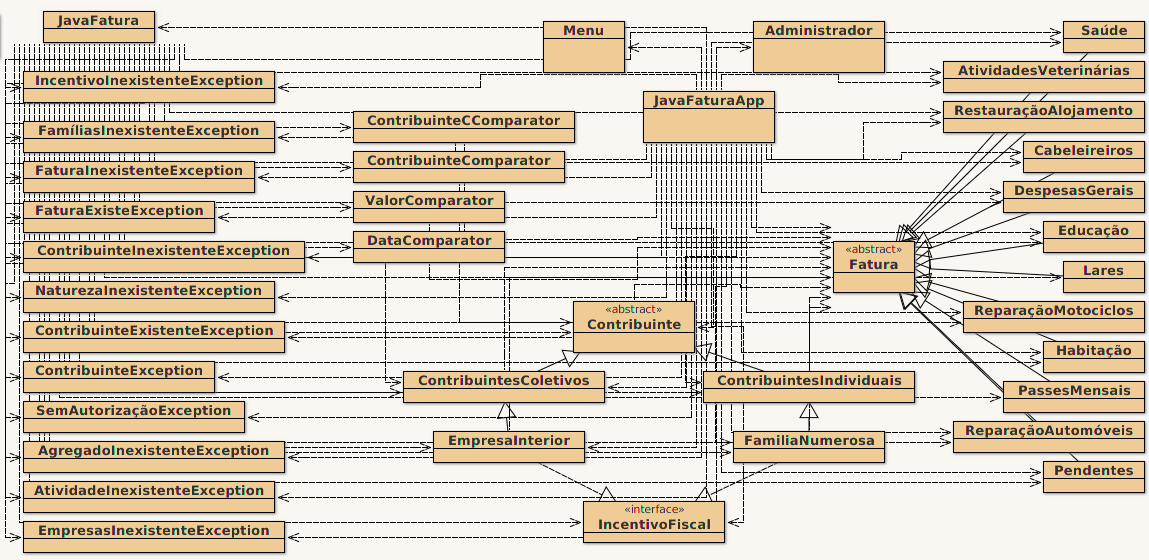
\includegraphics[width=15cm]{poo}\\
\end{center}

Nesta secção iremos abordar a estrutura da nossa aplicação, referindo as classes presentes, os atribuitos e o modo de funcionamento de cada uma.

\subsection{JavaFaturaApp}

\begin{center}
\graphicspath{ {/home/jessica/Desktop/} }
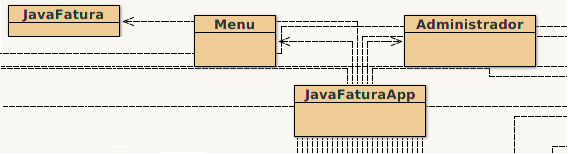
\includegraphics[width=10cm]{JavaFatura}\\
\end{center}

É a classe responsável por gravar o estado da aplicação e ler o mesmo de cada vez que a aplicação é fechada e reiniciada, respetivamente. Esta fornece uma interface ao utilizador que permite acesso às funcionalidades implementadas.\\

{\bf{Atributos}}

\begin{itemize}
 \item \textit{JavaFatura} javaFatura - Aplicação a correr
 \item \textit{Menu} menuInicial - Menu inicial
 \item \textit{Menu} menuContribuinteI - Menu para os contribuintes individuais
 \item \textit{Menu} menuContribuinteC - Menu para os contribuintes coletivos
 \item \textit{Menu} menuAdministrador - Menu para o administrador
 \item \textit{Menu} menuNatureza - Menu para a atividade económica
 \item \textit{Administrador} administrador - Administrador da aplicação
\end{itemize}

\subsubsection{Menu}

{\bf{Atributos}}\\

Esta classe é responsável pela criação e funcionamento dos menus. 

\begin{itemize}
 \item \textit{List$<$String$>$} opcoes - Lista as opções do menu
 \item \textit{int} op - Opção selecionada pelo utilizador
\end{itemize}

\subsection{JavaFatura}
\label{sec:solucao}

{\bf{Atributos}}\\

Esta classe é responsável pelo funcionamento da aplicação. É nesta que se encontram todas as funcionalidades implementadas, o que a torna uma das classes fundamentais do nosso projeto. 

\begin{itemize}
 \item \textit{Map$<$String,Contribuinte$>$} contribuintes - Lista dos utilizadores registados na aplicação
 \item \textit{List$<$String$>$} concelhos - Lista dos concelhos do interior
 \item \textit{Contribuinte} contribuinte - Utilizador com sessão iniciada
 \item \textit{int} id - Id da próxima fatura a ser registada
\end{itemize}

Para armazenar os contribuintes registados recorremos a uma \textit{TreeMap} cujo fator de comparação é o nif do utilizador. Esta escolha deveu-se à simples implementação e eficiente procura. Temos também num \textit{ArrayList} os concelhos com incentivo fiscal, visto que não será necessário aceder a nenhum concelho diretamente. Para facilitar a procura de uma fatura no momento do registo associamo-lhe um identificador (\textit{id}). 

\subsection{Contribuinte}
\label{sec:solucao}

\begin{center}
\graphicspath{ {/home/jessica/Desktop/} }
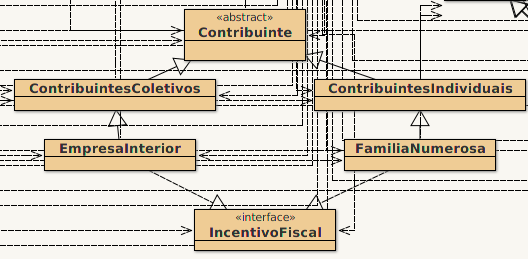
\includegraphics[width=10cm]{Contribuintes}\\
\end{center}

{\bf{Atributos}}\\

Classe abstrata com todos os atributos e métodos comuns a todos os diferentes tipos de utilizadores. 

\begin{itemize}
 \item \textit{String} nif - Número de identificação fiscal
 \item \textit{String} email - Email do contribuinte
 \item \textit{String} nome - Nome do contribuinte
 \item \textit{String} morada - Morada do contribuinte
 \item \textit{String} password - Password do contribuinte
 \item \textit{Map$<$String,Fatura$>$} faturas - Lista das faturas com atividade económica associada emitidas em nome do contribuinte
 \item \textit{Map$<$String,Fatura$>$} pendentes - Lista das faturas pendentes emitidas em nome do contribuinte
 \item \textit{double} despesa -  Despesa até ao momento do contribuinte
\end{itemize}

Dado que as faturas em estado pendente não são consideradas para efeitos de deduções, sentimos a necessidade de armazená-las numa estrutura diferente das que têm uma atividade económica associada. Para ambas implementamos uma \textit{HashMap} ordenada pelo seu id, dado que esta estrutura permite o endereçamento direto, o que a torna bastante eficaz. Para a implementação de um requesito tornou-se imperativo guardar a despesa do contribuinte até ao momento. Os restantes atributos são indespensáveis e característicos de cada contribuinte.

\subsubsection{Contribuintes Individuais}

Esta classe corresponde a um contribuinte individual que herda os parâmentros da classe anterior.\\

{\bf{Atributos}}
\begin{itemize}
 \item \textit{int} dependentes - Número de dependentes
 \item \textit{List$<$String$>$} nifs - Nif dos dependentes
 \item \textit{double} coeffiscal - Coeficiente fiscal
 \item \textit{List$<$String$>$} codigos - Códigos das atividades ecónomicas
 \item \textit{int} numFilhos - Número de filhos do contribuinte
\end{itemize}

Além dos elementos comuns à super classe acrescentamos o número de filhos para definição de uma família numerosa e as características específicas do contribuinte individual.

\subsubsection{FamiliaNumerosa}
Classe que além dos parâmetros herdados acrescenta a redução que será utilizada no cálculo da dedução fiscal.\\

{\bf{Atributos}}
\begin{itemize}
 \item \textit{double} reduçao - Bonificação
\end{itemize}

\subsubsection{Contribuintes Coletivos}

Esta classe corresponde a um contribuinte coletivo que adquire os parâmentros da super classe.\\

{\bf{Atributos}}
\begin{itemize}
 \item \textit{List$<$String$>$} atividadeEcon - Atividades em que a empresa atua
 \item \textit{double} fator - Fator que a empresa tem no cálculo de dedução fiscal
 \item \textit{Map$<$String,Fatura$>$} emitidas - Lista das faturas emitidas pelo contribuinte
 \item \textit{double} faturado - Valor faturado até ao momento
 \item \textit{String} concelho - Concelho do contribuinte
\end{itemize}

Além dos elementos comuns à super classe acrescentamos o concelho para determinar uma empresa do interior, as características específicas do contribuinte coletivo, o valor faturado até ao momento para a resolução de um requesito e \textit{HashMap} com as faturas registadas por este contribuinte.

\subsubsection{EmpresaInterior}
Classe que além dos parâmetros herdados acrescenta a redução que será utilizada no cálculo da dedução fiscal.\\

{\bf{Atributos}}
\begin{itemize}
 \item \textit{double} reduçao - Bonificação
\end{itemize}

\subsubsection{IncentivoFiscal}
Esta classe é uma interface que possiu as assinaturas dos métodos que permitem obter e alterar a redução.

\subsection{Fatura}


\begin{center}
\graphicspath{ {/home/jessica/Desktop/} }
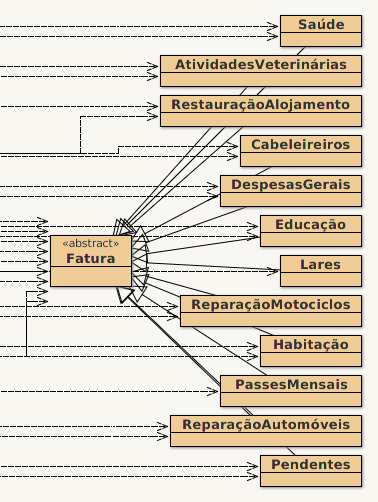
\includegraphics[width=6cm]{Faturas}\\
\end{center}

Classe abstrata com todos os atributos e métodos comuns aos diferentes tipos de fatura.\\

{\bf{Atributos}}
\begin{itemize}
 \item \textit{int} correção - Indica se a fatura foi alterada
 \item \textit{String} idFatura - Identificador da fatura
 \item \textit{String} nifEmitente - Número fiscal do emitente
 \item \textit{String} desig - Designação do emitente
 \item \textit{LocalDate} dataDespesa - Data da despesa 
 \item \textit{String} nifCliente - Número fiscal do cliente
 \item \textit{String} descricao - Descrição da despesa
 \item \textit{String} natureza - Natureza da despesa
 \item \textit{double} valor - Valor da despesa
\end{itemize}

Para rastrear as faturas em que a atividade económica foi modificada associamo-lhe uma variável (\textit{correção}) que possui o valor um caso tal se verifique. Os restantes atributos são os característicos da fatura.

\subsubsection{Saúde}

Classe correspondente a uma fatura do tipo Saúde, que além dos atributos herdados acrescenta a taxa a aplicar e o limite de dedução.\\

{\bf{Atributos}}
\begin{itemize}
 \item \textit{double} taxa - Taxa a aplicar
 \item \textit{int} limite - Limite máximo de dedução
\end{itemize}

\subsubsection{Educação}

Classe correspondente a uma fatura do tipo Educação, que além dos atributos herdados acrescenta a taxa a aplicar e o limite de dedução.\\

{\bf{Atributos}}
\begin{itemize}
 \item \textit{double} taxa - Taxa a aplicar
 \item \textit{int} limite - Limite máximo de dedução
\end{itemize}

\subsubsection{Lares}

Classe correspondente a uma fatura do tipo Lares, que além dos atributos herdados acrescenta a taxa a aplicar e o limite de dedução.\\

{\bf{Atributos}}
\begin{itemize}
 \item \textit{double} taxa - Taxa a aplicar
 \item \textit{int} limite - Limite máximo de dedução
\end{itemize}

\subsubsection{RestauraçãoAlojamento}

Classe correspondente a uma fatura do tipo Restauração e Alojamento, que além dos atributos herdados acrescenta a taxa a aplicar e o limite de dedução.\\

{\bf{Atributos}}
\begin{itemize}
 \item \textit{double} taxa - Taxa a aplicar
 \item \textit{int} limite - Limite máximo de dedução
\end{itemize}

\subsubsection{ReparaçãoAutomóveis}

Classe correspondente a uma fatura do tipo Reparação de Automóveis, que além dos atributos herdados acrescenta a taxa a aplicar e o limite de dedução.\\

{\bf{Atributos}}
\begin{itemize}
 \item \textit{double} taxa - Taxa a aplicar
 \item \textit{int} limite - Limite máximo de dedução
\end{itemize}

\subsubsection{ReparaçãoMotociclos}

Classe correspondente a uma fatura do tipo Reparação de motociclos, que além dos atributos herdados acrescenta a taxa a aplicar e o limite de dedução.\\

{\bf{Atributos}}
\begin{itemize}
 \item \textit{double} taxa - Taxa a aplicar
 \item \textit{int} limite - Limite máximo de dedução
\end{itemize}

\subsubsection{Cabeleireiros}

Classe correspondente a uma fatura do tipo Cabeleireiros , que além dos atributos herdados acrescenta a taxa a aplicar e o limite de dedução.\\

{\bf{Atributos}}
\begin{itemize}
 \item \textit{double} taxa - Taxa a aplicar
 \item \textit{int} limite - Limite máximo de dedução
\end{itemize}

\subsubsection{DespesasGerais}

Classe correspondente a uma fatura do tipo Despesas Gerais, que além dos atributos herdados acrescenta a taxa a aplicar e o limite de dedução. \\

{\bf{Atributos}}
\begin{itemize}
 \item \textit{double} taxa - Taxa a aplicar
 \item \textit{int} limite - Limite máximo de dedução
\end{itemize}

\subsubsection{PassesMensais}

Classe correspondente a uma fatura do tipo Passes Mensais, que além dos atributos herdados acrescenta a taxa a aplicar e o limite de dedução. \\

{\bf{Atributos}}
\begin{itemize}
 \item \textit{double} taxa - Taxa a aplicar
 \item \textit{int} limite - Limite máximo de dedução
\end{itemize}

\subsubsection{AtividadesVeterinárias}

Classe correspondente a uma fatura do tipo Atividades Veterinárias, que além dos atributos herdados acrescenta a taxa a aplicar e o limite de dedução. \\

{\bf{Atributos}}
\begin{itemize}
 \item \textit{double} taxa - Taxa a aplicar
 \item \textit{int} limite - Limite máximo de dedução
\end{itemize}

\subsubsection{Habitação}

Classe correspondente a uma fatura do tipo Habitação, que além dos atributos herdados acrescenta a taxa a aplicar e o limite de dedução. \\

{\bf{Atributos}}
\begin{itemize}
 \item \textit{double} taxa - Taxa a aplicar
 \item \textit{int} limite - Limite máximo de dedução
\end{itemize}

\subsubsection{Pendentes}
Classe que não acrescenta nenhum atributo aos herdados da super classe.

\subsection{Exceptions}

\begin{center}
\graphicspath{ {/home/jessica/Desktop/} }
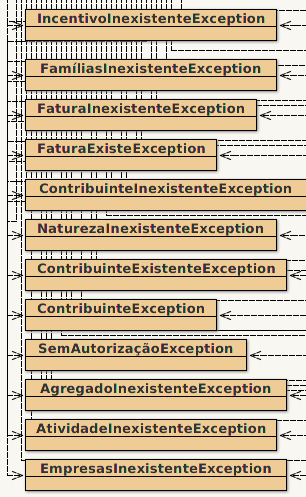
\includegraphics[width=5cm]{EX}\\
\end{center}

Para o caso de não existir nenhum elemento requerido, tornou-se imperativo a utilização de exceções que permitem solucionar este problema.\\
\begin{itemize}
 \item FaturaInexistenteException
 \item FaturaExisteException
 \item ContribuinteInexistenteException
 \item NaturezaInexistenteException
 \item ContribuinteExistenteException
 \item ContribuinteException
 \item SemAutorizaçãoException
 \item AgregadoInexistenteException
 \item AtividadeInexistenteException 
\end{itemize}

\cleardoublepage

\section{Descrição da aplicação}
\label{sec:solucao}
A aplicação disponibiliza ao utilizador uma interface de fácil utilização, que funciona à base de opções por números. Quando o utilizador executa a aplicação é lhe apresentado o seguinte menu:

\begin{center}
\graphicspath{ {/home/jessica/Desktop/} }
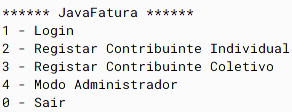
\includegraphics[width=6cm]{MenuLogin}\\
\end{center}


Neste menu inicial o contribuinte pode registar-se na \textit{Opção 2} na eventualidade de ser um contribuinte individual ou na \textit{Opção 3} se for coletivo. Para o administrador aceder à aplicação terá de selecionar a \textit{Opção 4}. Se o utilizador efetuar o registo, terá de inserir algumas informações como nos exemplos:


\graphicspath{ {/home/jessica/Desktop/} }
\begin{center}
	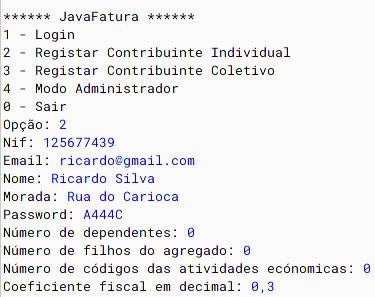
\includegraphics[height=5cm]{MenuRCI}  \quad
	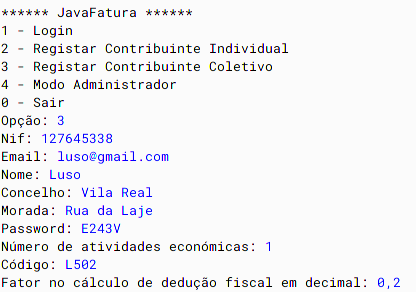
\includegraphics[height=5cm]{MenuRCC}
\end{center}

Na nossa aplicação assumimos que os utilizadores tem acesso a uma tabela com os códigos correspondentes às diferentes atividades económicas existentes que será útil aquando do registo na aplicação: \\

{\bf{\textcolor{Maroon}{Cabeleireiros}}} C201\\
\indent {\bf{\textcolor{Maroon}{Lares}}} L502\\
\indent {\bf{\textcolor{Maroon}{Passes Mensais}}} PM354\\
\indent {\bf{\textcolor{Maroon}{Educação}}} E478\\
\indent {\bf{\textcolor{Maroon}{DespesasGerais}}} DG678\\
\indent {\bf{\textcolor{Maroon}{Restauração e Alojamento}}} RA897\\
\indent {\bf{\textcolor{Maroon}{Atividades Veterinárias}}} AV292\\
\indent {\bf{\textcolor{Maroon}{Habitação}}} H512\\
\indent {\bf{\textcolor{Maroon}{Reparação Automóveis}}} RA1278\\
\indent {\bf{\textcolor{Maroon}{ReparaçãoMotociclos}}} RM333\\
\indent {\bf{\textcolor{Maroon}{Saúde}}} S126\\


Estando registado o utilizador pode fazer o login na \textit{Opção 1}, como apresentamos de seguida:

\begin{center}
\graphicspath{ {/home/jessica/Desktop/} }
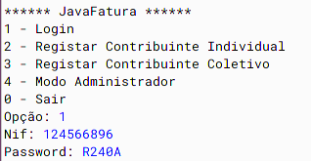
\includegraphics[width=7cm]{MenuLoginC}\\
\end{center}

No caso de o utilizador iniciar sessão como contribuinte individual, será apresentado o menu com todos as funcionalidades disponiveis na aplicação:

\begin{center}
\graphicspath{ {/home/jessica/Desktop/} }
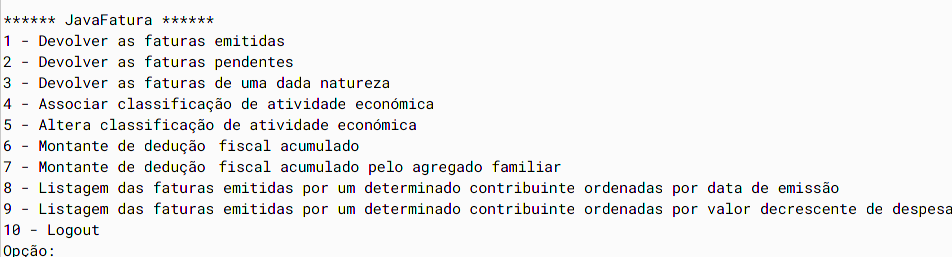
\includegraphics[width=16cm]{MenuCI}\\
\end{center}

\begin{itemize}
 \item 1. Esta opção permite ao utilizador visualizar as faturas emitidas em seu nome com uma atividade económica associada
 \item 2. Faculta as faturas em que é necessário associar a atividade económica
 \item 3. Devolve todas as faturas com uma dada atividade económica
 \item 4. Atribui a uma dada fatura pendente a atividade económica
 \item 5. Altera a atividade económica de uma dada fatura
 \item 6. Devolve o montante de dedução fiscal acumulado pelo contribuinte
 \item 7. Devolve o montante de dedução fiscal acumulado pelo contribuinte e seu agregado
 \item 8. Lista as faturas emitidas por um determinado contribuinte coletivo ordenadas por data de emissão
 \item 9. Lista as faturas emitidas por um determinado contribuinte coletivo ordenadas por valor decrescente de despesa
 \item 10. Permite terminar a sessão na aplicação
\end{itemize}

Na eventualidade de ser um contribuinte coletivo, o menu fornecido será:

\begin{center}
\graphicspath{ {/home/jessica/Desktop/} }
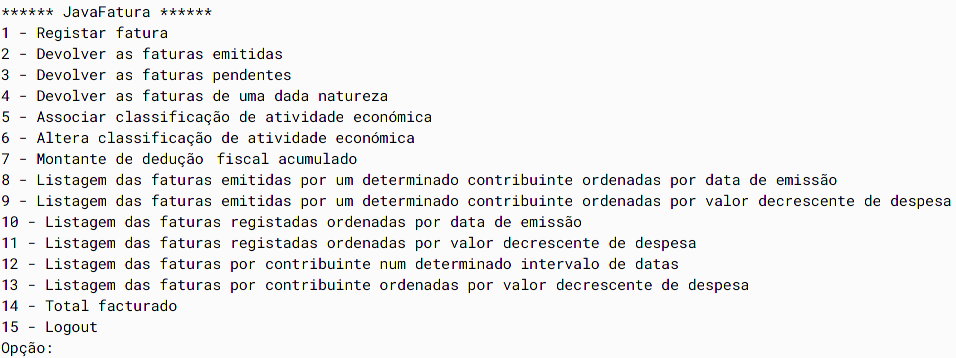
\includegraphics[width=16cm]{MenuCC}\\
\end{center}

\begin{itemize}
 \item 1. Possibilita registar uma fatura em nome de um contribuinte\\

 Quando esta opção for selecionada o utilizador irá se deparar com o seguinte estado da aplicação:

\begin{center}
\graphicspath{ {/home/jessica/Desktop/} }
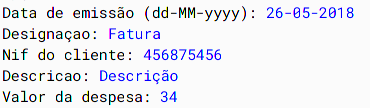
\includegraphics[width=7cm]{RegistarFatura}\\
\end{center}

 \item 2. Esta opção permite ao utilizador visualizar as faturas emitidas em seu nome com uma atividade económica associada
 \item 3. Faculta as faturas em que é necessário associar a atividade económica
 \item 4. Devolve todas as faturas com uma dada atividade económica
 \item 5. Atribui a uma dada fatura pendente a atividade económica
 \item 6. Altera a atividade económica de uma dada fatura
 \item 7. Devolve o montante de dedução fiscal acumulado pelo contribuinte
  \item 8. Lista as faturas emitidas por um determinado contribuinte coletivo ordenadas por data de emissão
 \item 9. Lista as faturas emitidas por um determinado contribuinte coletivo ordenadas por valor decrescente de despesa
 \item 10. Lista todas as faturas registadas pelo contribuinte ordenadas pela data de emissão
 \item 11. Devolve todas as faturas registadas pelo contribuinte por valor decrescente de despesa
 \item 12. Lista todas as faturas registadas em nome de um dado contribuinte no intervalo de datas solicitado
 \item 13. Devolve todas as faturas registadas em nome de um dado contribuinte por valor decrescente de despesa
 \item 14. Retorna o total faturado pela empresa
 \item 15. Permite terminar a sessão na aplicação
\end{itemize}


Tanto os contribuinte individuais como os contribuintes coletivos tem disponível a funcionalidade de alterar ou associar uma atividade económica a uma fatura, desta forma quando uma destas opções for requerida ser-lhe-á permitido selecionar qual a atividade que pretende, como podemos verificar de seguida: 

\begin{center}
\graphicspath{ {/home/jessica/Desktop/} }
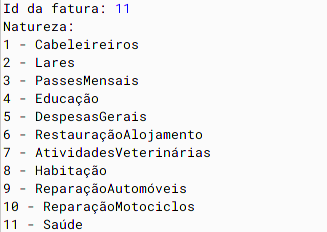
\includegraphics[width=8cm]{MenuNatureza}\\
\end{center}

Em último caso, se for o adminstrador a aceder à aplicação é lhe pedido o código de acesso: 

\begin{center}
\graphicspath{ {/home/jessica/Desktop/} }
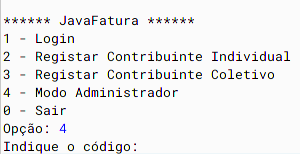
\includegraphics[width=7cm]{MenuLoginAdmin}\\
\end{center}

De seguida ser-lhe-á disponível o seguinte menu, com funcionalidades únicas:

\begin{center}
\graphicspath{ {/home/jessica/Desktop/} }
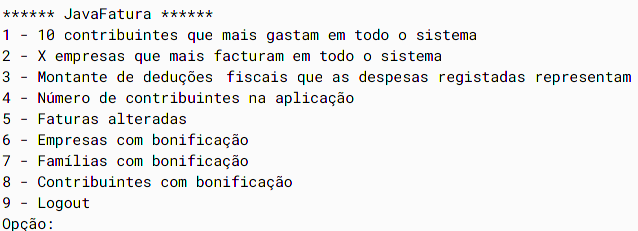
\includegraphics[width=15cm]{MenuAdmin}\\
\end{center}

\begin{itemize}
 \item 1. Lista os 10 contribuintes que mais gastam em todo o sistema
 \item 2. Devolve os X contribuintes coletivos que mais faturam em todo o sistema
 \item 3. Permite obter o montante de dedução fiscal das X empresas que mais faturam no sistema
 \item 4. Apresenta o número de contribuintes coletivos e individuais registados na aplicação
 \item 5. Faculta todas as faturas cuja a atividade económica foi alterada pelos contribuintes
 \item 6. Lista todos os contribuintes coletivos situados no interior do país e que por isso têm benefício fiscal
 \item 7. Devolve todos os contribuintes individuais que têm mais que quatro filhos tendo assim uma bonificação
 \item 8. Devolve todos os contribuintes com benefício fiscal
 \item 9. Permite terminar a sessão na aplicação
\end{itemize}

\cleardoublepage

\section{Inclusão de novos conceitos}
\label{sec:solucao}
Apesar de considerarmos que a nossa aplicação suporta quase todo o tipo de despesas, elaboramo-la de modo que a inclusão de novos tipos seja bastante simples. Para tal, apenas teriamos de criar uma classe que herdasse todos os atributos e métodos da classe abstrata \textit{Fatura}.\\

{\bf{Algoritmo de cálculo de dedução fiscal implementado na aplicação}}\\

As diferentes atividades económicas apresentam uma limite máximo e uma taxa características de cada. Assim sendo, para o cálculo de dedução fiscal de ambos os contribuintes tornou-se imperativo multiplicar o valor da despesa pela taxa correspondente à sua natureza e ir somando o valor das deduções de uma mesma atividade e no caso de esse exceder o limite, consideramos o valor deduzido o limite.\\
\indent Na possibilidade de o contribuinte ser coletivo, ao valor deduzido somamos o fator que a empresa tem no cálculo de dedução fiscal a multiplicar pelo deduzido. Na eventualidade de o contribuinte ser individual, ao valor deduzido somamos o coeficiente fiscal para efeitos de dedução a multiplicar pelo deduzido. Se o contribuinte individual tiver mais de quatro filhos o limite na área da saúde e das despesas gerais aumenta em 5\% por cada filho. Caso o contribuinte coletivo se situe num concelho do interior, aumentamos 20\% do valor deduzido.\\
\indent De modo a tornar o algoritmo mais completo, poderíamos aplicar a bonificação de uma familia numerosa aos filhos e não aos pais (como é realizado). Outra hipótese seria apenas permitir ao contribuinte deduzir as despesas para os quais os seus códigos permitiam, no entanto consideramos que todos os contribuintes deverão ter o direito de deduzir para todas as diferentes atividades económicas.

\cleardoublepage

\section{Conclusão}
\label{sec:conclusao}
Este projeto permitiu-nos desenvolver novas capacidades enquanto programadores, uma vez que é a primeira vez que lidamos com programação orientada a objetos. Muitos dos problemas com os quais nos deparamos deveram-se a esta alteração de paradigma, no entanto com trabalho foram solucionados. 

Em última instância, consideramos que os nossos objetivos neste projeto foram alcançados, contudo ainda podiam ser melhorados alguns aspetos, nomeadamente a disponibilização de mais funcionalidades na aplicação e a organização de código.

\end{document}
\grid
\grid
\grid
